\section{Le 6 W}

Un sito web lo possiamo considerare come un negozio. Prima di entrare in un nuovo negozio l'approccio comune consiste nel guardare la \textbf{vetrina}. Questo è un punto cruciale, perchè è proprio in quel momento che decidiamo se entrare in un negozio oppure proseguire oltre. Questo avviene per il web esattamente allo stesso modo. La homepage in questo contesto è la vetrina del negozio. Come si può immaginare è impossibile o comunque poco ragionevole mostrare l'intero contenuto del negozio nella sua vetrina. Lo scopo del commerciante è quello di far sì che l'utente entri nel suo negozio, per cui è necessario attirare la sua attenzione e suscitare la sua curiosità. Le apparenze in questo campo sono molto importanti. Il proprietario del sito web deve pertanto cercare di soddisfare le cosiddette 6 W.

Supponiamo di essere un utente indefinito, non necessariamente appassionato di informatica o di sviluppo web ma comunque con un grado minimo di intelligenza e cultura. A Nel momento in cui io capito \textbf{casualmente} per la prima volta su html.it quello che vedo è rappresentato dalla figura seguente:

\begin{figure}[htpd]
\centering
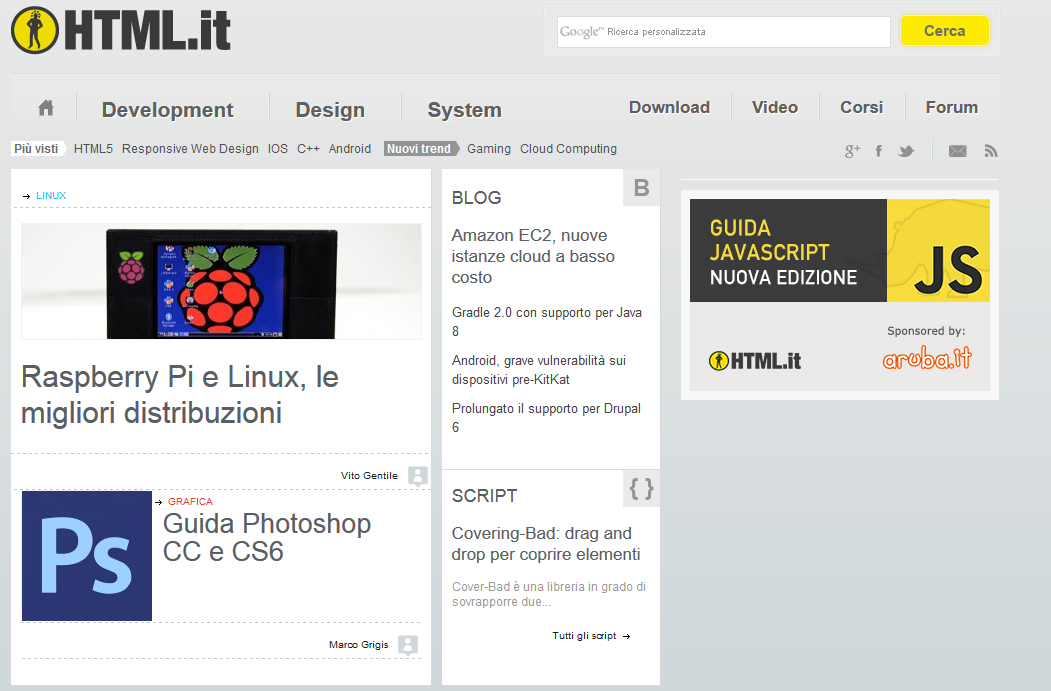
\includegraphics[width=120mm]{images/home.png}
\caption{La home page di html.it}
\end{figure}

Ho eseguito una serie di test ad una persona corrispondente al profilo indicato. Ho dato ad essa un tempo compreso tra i 10 e i 30 secondi e le ho detto di porsi le seguenti domande:

\subsection{Where?}

\begin{center}

\textit{A che tipo di sito sono arrivato? Quale contenuto mi offre?}

\end{center}

Il soggetto ha riconosciuto in tempi brevi che il sito si occupa di informatica e che offre la visualizzazione di articoli e guide. Ciò è stato possibile grazie alla presenza degli ultimi articoli direttamente nella home page. In questo modo è comprensibile a primo sguardo di cosa il sito tratta, per cui se il soggetto fosse stato interessato a leggere un articolo o una guida sull'argomento molto probabilmente avrebbe continuato la navigazione nel sito.

\subsection{Who?}

\textit{Chi rappresenta il sito?}

\subsection{Why?}

\textit{Perchè mai dovrei fermarmi su questo sito? Quali benefici mi porta?}

\subsection{What?}

\textit{Cosa offre il sito?}

\subsection{When?}

\textit{Quali sono le ultime novità? Quando è stato manutenuto per l'ultima volta?}

\subsection{How?}

\textit{Come faccio ad arrivare alle sezioni principali?}



